\documentclass[12pt]{book} 

\usepackage{amsmath}
\usepackage{graphicx}
\usepackage{import}

\setlength{\parindent}{0em}  % sets auto indent at new paragraph to none

\newcommand{\incfig}[1]{%
    \import{./figures/}{#1.pdf_tex}
}

\title{\coursetitle\linebreak\lecturename}
\author{\\Cain Susko\\ 
           \\ \\ \\
      Queen's University 
    \\School of Computing\\} 

%=-=-=-=-=-title-=-=-=-=-=%
\newcommand{\lecturename}{A Wold of Cities}
\newcommand{\coursetitle}{Urban Planning}
%=-=-=-=-=-#####-=-=-=-=-=%

\begin{document}
\begin{titlepage}
        \maketitle
\end{titlepage}


\section*{The Urban and The Global}
Cities are connected not only within a region but globally.
This is because of the growth of global trade (like NAFTA) in the 90's which reshaped economic geographies as manufacturing could move
        more easily and jobs and companies became more globally integrated.

For example, the investment in Canada has increased steadily, and thus the Canadian market is also a global market. 
Like how the Toronto real estate market has both local and foreign buyers.
Another example is of whistler, which is implicitly connected to the global economy as it is a tourist town.

This globalized economy requires alot of effort and work (for example, the EverGiven in the Suez Canal) to maintain and this work is also required in cities as they become more globalized.

In summary, the Global affects the Urban and the lives lived within it.

\section*{Global and World Cities}
there are 2 ways of analyzing cities in the context of the world:
\begin{itemize}
        \item the World City approach
        \item the Global City approach
\end{itemize}

As economic globalization accelerated geographers and other social scientists tried
to understand how these global economic connections shape cities and economic
activity
\pagebreak

\subsection*{World Cities}
The World approach, coined by Friedman and Wolff, began to describe what roles specific cities began to take on in the 
        growing global economy.
These roles were thought of by F and W as the command and control functions cities used to coordinate the global
        trade connected to it.
It can almost be thought of as an urban hierarchy of influence and control.

The World Cities approach can be illustrated on a map like so:
\begin{figure}[h]
        \centering
        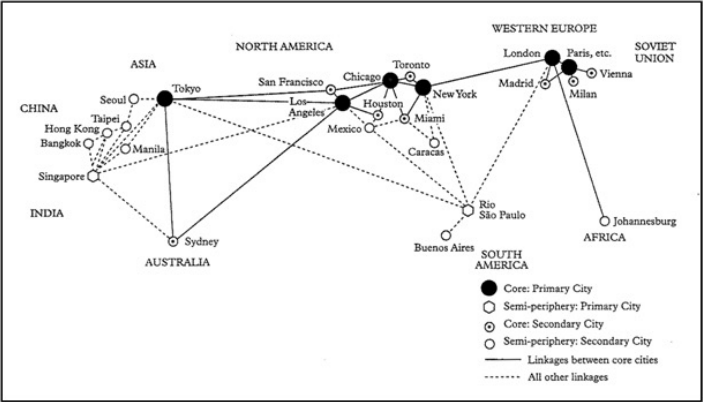
\includegraphics[scale=0.5]{./figures/wcitymap.png}
\end{figure}

\subsection*{Global Cities}
The Global approach is an extension of the World approach by Sassen by focusing on how global cities are characterized by inequality. 
It advanced the understanding of how cities interconnect by stating that these cities with command and control functions operate as 
        a system that provides Advanced Producer Services.

This is to say that the cities and functions have become so complex that they require other ancilliary functions to operate.
For example, a large international banking firm needs a plethora of other services that can be provided by the city.
The global city thus is only possible by the local individuals in each city that may not be benifitting from the global investment
        that is shaping their city.
\pagebreak

\paragraph{}
When cities are a part of these world/global networks they are changed by eachother
\begin{itemize}
        \item they compete with eachother
        \item they have to balance local and global interests.
        \item they become homogeneous 
        \item they become less intertwined with their surrounding area
\end{itemize}

In summary, the world/global cities theories draw attention to the global connections linking cities and how they affect eachother.
The place in the hierarchy a city is in effects itsself and its citizens.

\section*{The Global Beyond the Economic}
The usual metric used to determine if a city is 'global' it its economic prowess. 
This leaves many cities--particularly in the south--off the map.

Furthermore, there are questions of if this idea of global cities is even new (colonialism\ldots).
Additionally, there are a variety of 'global flows' that connect cities to others around the world that shapes the city.
These include
\begin{itemize}
        \item consumer products
        \item intermediate services
        \item people
        \item finance
        \item information and ideas
        \item nasty flows
\end{itemize}

\subsection*{Policy Mobilities}
As information is spread through flows of cities, ideas on how a city should be run flow through as well.
Such policies are neither local nor global but made through mutations as the ideas travel.

An example of such a policy is that of the 'Creative City' which addresses the idea that if a city attracted creatives,
        they could grow and develop. In London and Bandung, these cities worked together to implement Creative City policy
        and thus, they had similar policy.

In summary, there can be may 'flows' that effect cities in important ways other than just economic factors.


\section*{Ordinary and Worlding Cities}
While there are many metrics of measuring globalness in a city, it is important to distinguish which measures are more important.
There are 2 theories for this ordering of flows:
\begin{itemize}
        \item Ordinary cities
        \item Worlding cities
\end{itemize}

\subsection*{Ordinary}
Ordinary theory states that one should focus on 'ordinary' cities when researching global connectedness in order to get a more
        accurate gauge of how the general world is connected.

\subsection*{Worlding}
Worlding theory states The distinctive experiences of the cities of the global South can generate productive
        and provocative theoretical frameworks for all cities. 
For example, the actions being taken in the south by slum-dwellers to improve their quality of life is a template that can be 
        used to reclaim and improve the dilapitated suburbs of Chicago.

\paragraph{}
both these theories focus on the cities that have generally been kept 'off the map' in other global analysis.
It also removes the analysis from the influence of \textit{Global Elites} which allows for results that are more accurate
        to the local people.
\end{document}

